\documentclass{article}
\usepackage{url}
\usepackage{graphicx}
\usepackage{float}
\usepackage{biblatex}
\addbibresource{ref.bib}
\graphicspath{{./images}}
\title{Analysis of Sample2.exe \\Practical Assignment 2\\Malware Reverse Engineering \\
CAP6137}
\author{Michael Ivanov \\
ivanovmichael@ufl.edu}
\date{March 14, 2022}

\begin{document}
    \maketitle
    \pagebreak
    \section{Executive Summary}
    This malware belongs in the \textit{TrickBot} family. The malware bundles encoded files inside its program section. By examining the disassembly you can see these resource files being loaded and then later modified. They are decoded by using the XOR operation of each byte in a loop. By using a debugger such as \textit{x32dbg} I was able to pause execution after the decoding and dump the contents of memory into a file. This dumped file is now the decoded resource. This malware is able to dynamically run function by using \textit{GetProcAddress} which allows it to use these obfuscated resource functions. The dumped binary provides various networking and cryptographic functions. The malware spreads to several system directories before deleting its current location. The malware sends an HTTP request to \url{http://myexternalip.com/raw} in order to find the machines external IP. Running the dumped decoded binary on its own gives us some more network behaviors. It will connect to \url{in-addr.arpa} to preform a reverse DNS lookup. The malware is a 32 bit executable, but it is able to  access system32 by using the \textit{Heaven's gate} hooking method.
    \pagebreak
    \section{Static Analysis}
    \subsection{MD5 Hashes}
    \begin{itemize}
        \item sample2.exe: E05D85ACC62B2795BFB94A681E64E20F
        \item resource1 IDR{\_}X86BOT: 958596F72BD381520A75FFA6E4DB9827
        \item resource2 IDR{\_}X86LOADER: 27DA8F25FF1CB54C63618D2A489EE4DF
        \item resource3 IDR{\_}X86BOT: E8AF535C7447D203FF7CD44440B00459
        \item decoded IDR{\_}X86BOT: 1F1EDE22004510FB903D4CB45A769B12
    \end{itemize}

    \subsection{Program Compilation Date}
    \begin{itemize}
        \item sample2.exe: Fri Aug 19 09:54:32 2016
    \end{itemize}

    \subsection{Suspicious Imports}
    sample2.exe:
    \begin{itemize}
        \item \textbf{CreateProcessW:} This gives an indication the malware could be creating other processes.
        \item \textbf{VirtualProtect:} This can be used to change the permissions and protections of a process.
        \item \textbf{NtQueryInformationProcess:} Can be used to retrieve information about a specified process.
        \item \textbf{GetProcAddress:} This allows for run-time resolved function calls.
    \end{itemize}
    decoded.bin (IDR{\_}X86BOT):

    \begin{itemize}
        \item \textbf{winhttp.dll, iphlpapi.dll, ws2{\_}32.dll:} these DLLs provides many functions for networking.
        \item \textbf{crypt32.dll:} This DLL provides cryptographic messaging functions and may be used to encrypt network traffic or data.
    \end{itemize}

    \subsection{Suspicious Strings}
    \begin{itemize}
        \item \textbf{"Wow64DisableWow64FsRedirection":} A function that disables file system redirection for the calling thread. This could be used for the \textit{Heaven's Gate} hooking method \cite{Wow64}.
        \item \textbf{"FindResource", "LoadResource":} Functions for finding and loading an external resource.
        \item \textbf{"Sleep":} Might be useful to know for later dynamic analysis, the program might hang for a long period of time.
        \item \textbf{".log"} A possible file extension to some kind of log file.
    \end{itemize}

    \subsection{Program sections}
    In the .rsrc (resource) section there are 3 files. I have provided the hashes above.

    \subsection{Anti-disassembly}
    I was not able to find any indications of anti-disassembly.
    \subsection{Program obfuscation}
    \begin{figure}[H]
        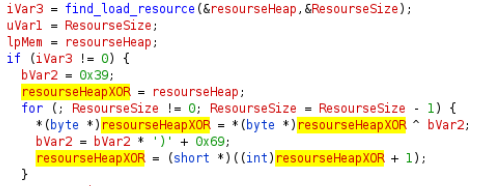
\includegraphics[width=\textwidth]{encodeXOR.png}
        \caption{Ghidra disassembly of potential resource obfuscation with XOR}
    \end{figure}

    \section{Dynamic Analysis}

    \subsection{Interesting behaviors}
    When the program is first executed it immediately deletes itself. However, by using Procmon I was able to see the program was still running. It was now in the \path{C:/Users/malware/AppData/Roaming} directory.
    \begin{figure}[H]
        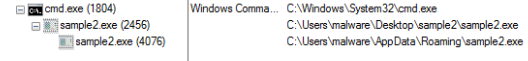
\includegraphics[width=\textwidth]{sample2process.png}
        \caption{Procmon showing the process tree of sample2.exe}
    \end{figure}
    The program uses \textit{GetProcAddress} to dynamically call \textit{Wow64DisableWow64FsRedirection}. This is a form of \textit{Heaven's Gate} hooking to allow the 32-bit application to gain access to native system32 directory\cite{gate}.
    \begin{figure}[H]
        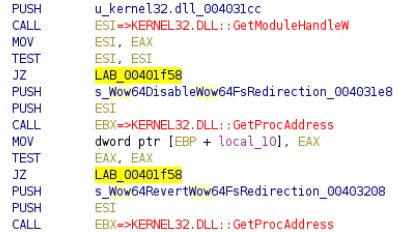
\includegraphics[width=\textwidth]{gate.png}
        \caption{An example of \textit{Heaven's Gate} hooking}
    \end{figure}

    \subsection{Contacted machines and services}
    \begin{itemize}
        \item HTTP GET \url{http://myexternalip.com/raw}
        \item TCP and DNS request \url{in-addr.arpa}
    \end{itemize}
    The above URL obtains the machine's external IP address. This may determine program behavior based on said IP address.
    \begin{figure}[H]
        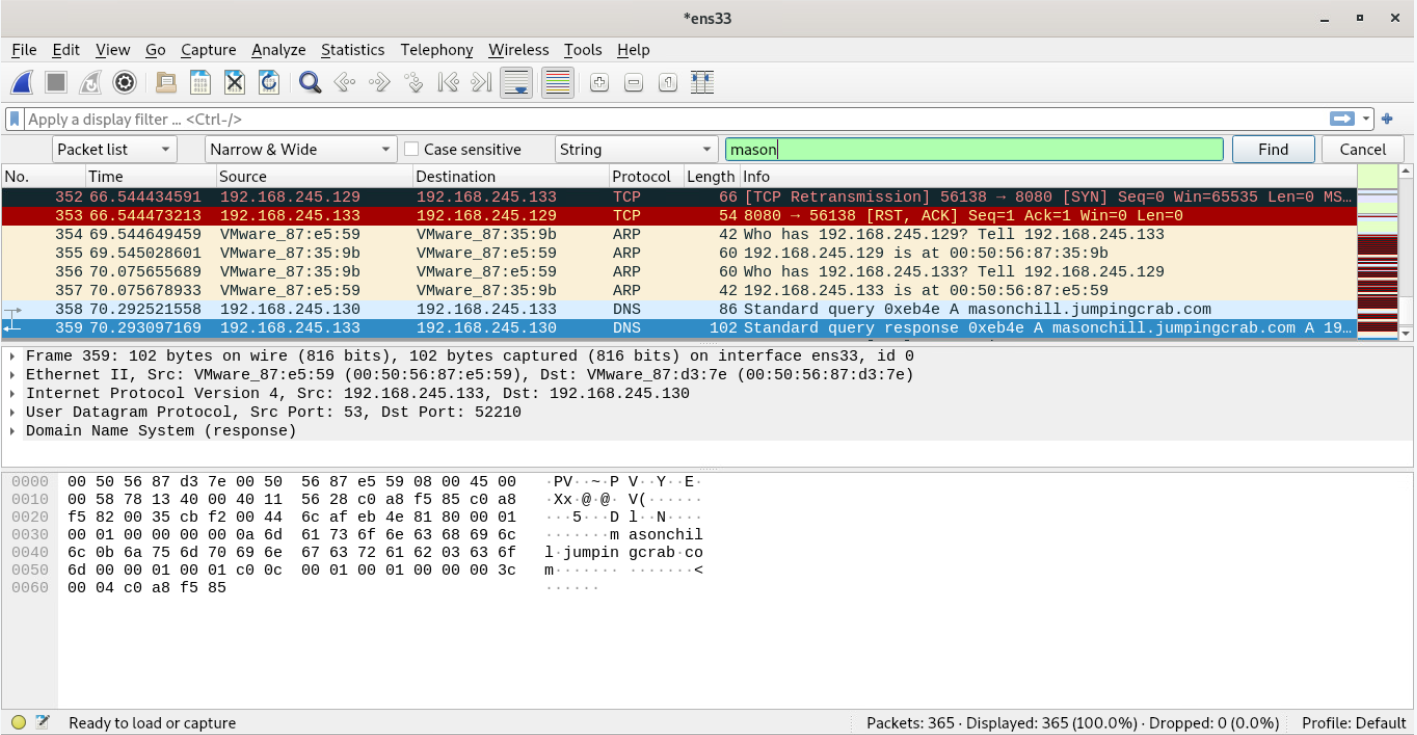
\includegraphics[width=\textwidth]{wireshark.png}
        \caption{Wireshark showing the HTTP get request from the above URL }
    \end{figure}
    \begin{figure}[H]
        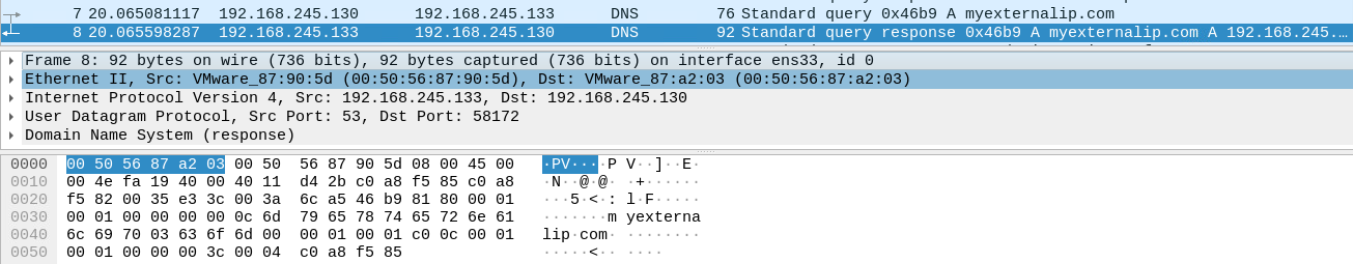
\includegraphics[width=\textwidth]{dns.png}
        \label{dns}
        \caption{Wireshark showing the DNS query and response }
    \end{figure}
    When running the decoded executable I was able to pick some TCP traffic to \url{in-addr.arpa}. Looking at the address online tells us this domain is used for Reverse DNS lookup\cite{rDNS}.
    \begin{figure}[H]
        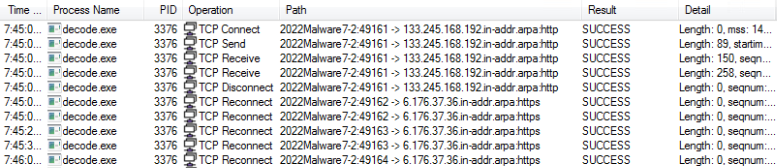
\includegraphics[width=\textwidth]{tcp.png}
        \label{dns}
        \caption{Procmon showing TCP traffic from the decoded executable}
    \end{figure}
    \begin{figure}[H]
        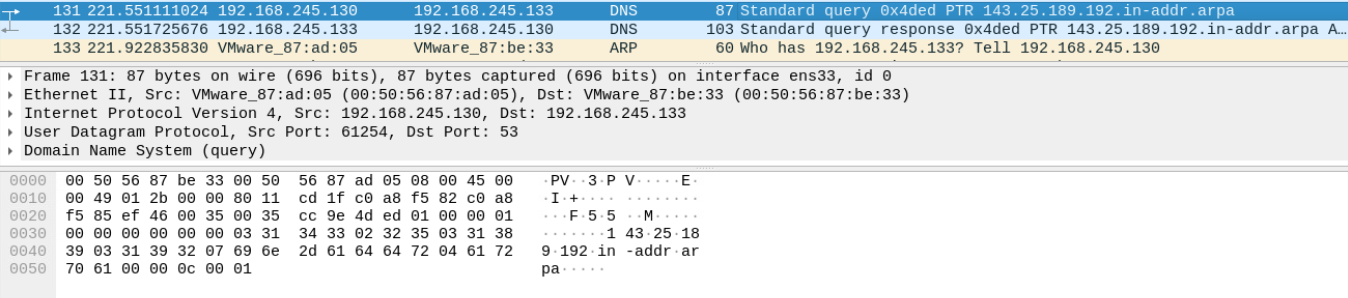
\includegraphics[width=\textwidth]{dns2.png}
        \label{dns}
        \caption{Wireshark showing the DNS query and response of the decoded executable}
    \end{figure}

    \subsection{Registry Keys created/modified}
    No registry keys were created or modified. However, the following key would have been created if it did not exist already.
    \begin{itemize}
        \item \path{HKLM\System\CurrentControlSet\Services\Tcpip\Parameters}
    \end{itemize}
    \begin{figure}[H]
        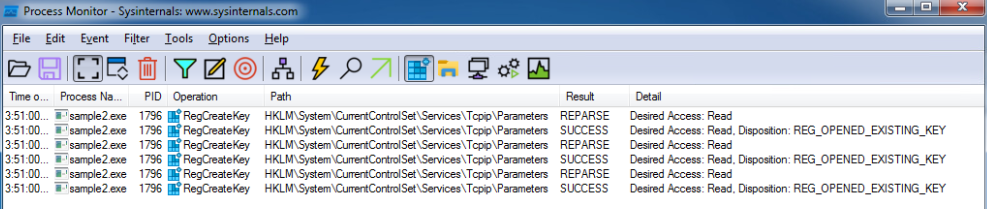
\includegraphics[width=\textwidth]{RegKeyCreate.png}
        \caption{Procmon showing the attempted creation of a registry key}
    \end{figure}

    \subsection{Files created/modified}
    Files Created:


    All instances of sample2.exe share the same hash.
    \begin{itemize}
        \item \path{C:\Users\malware\AppData\Roaming\sample2.exe}
        \item \path{C:\Users\System32\config\systemprofile\AppData\Roaming\sample2.exe}
        \item \path{C:\Users\System32\config\systemprofile\AppData\Roaming\client_id}
        \item \path{C:\Users\System32\config\systemprofile\AppData\Roaming\group_tag}
        \item \path{C:\Users\System32\config\systemprofile\AppData\Roaming\Modules}
    \end{itemize}
    \begin{figure}[H]
        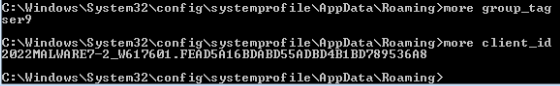
\includegraphics[width=\textwidth]{fileContents.png}
        \caption{The contents of the two new created files}
    \end{figure}
    \subsection{Processes started}
    \begin{itemize}
        \item \path{C:\Users\malware\AppData\Roaming\sample2.exe}
        \item \path{C:\Users\System32\config\systemprofile\AppData\Roaming\sample2.exe}
    \end{itemize}
    \begin{figure}[H]
        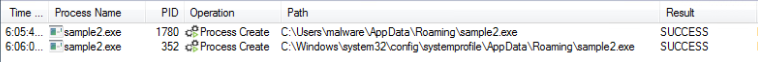
\includegraphics[width=\textwidth]{processCreated.png}
        \caption{Procmon showing the processes created by sample2.exe}
    \end{figure}

    \subsection{Persistence}
    On reboot, I was able to see the sample2.exe running in the background using process explorer. It was located in the \path{C:\Users\System32\config\systemprofile\AppData\Roaming} directory. It's parent process is the \textit{Task Scheduler Engine}.
    \begin{figure}[H]
        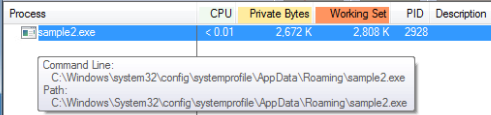
\includegraphics[width=\textwidth]{reboot.png}
        \caption{Procexp showing the malware running after a reboot}
    \end{figure}
    \begin{figure}[H]
        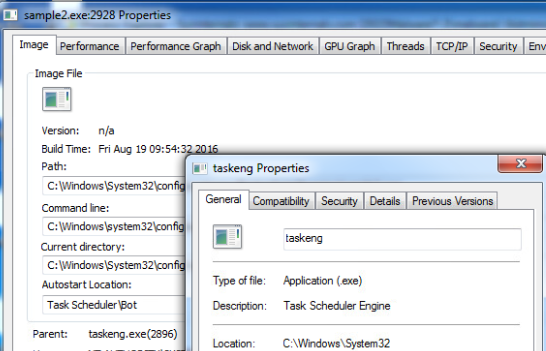
\includegraphics[width=\textwidth]{taskSced.png}
        \caption{The Task Scheduler Engine as the parent process}
    \end{figure}

    \subsection{Deobfuscation}
    As seen in the static analysis obfuscation section, there was a suspicious for loop in the main function with a XOR operation. By examining the previous functions I was able to conclude that this loop was decoding a resource file by the name of IDR{\_}X86BOT. By stopping the debugger after this loop and dumping the data from address EDI till size ECX I was able to decode the binary. 
    \begin{figure}[H]
        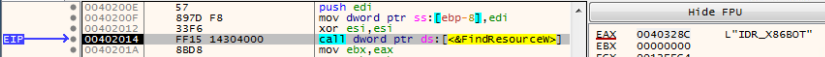
\includegraphics[width=\textwidth]{loadx86bot.png}
        \caption{Find and load of the encoded IDR{\_}X86BOT resource to be decoded later}
    \end{figure}
    \begin{figure}[H]
        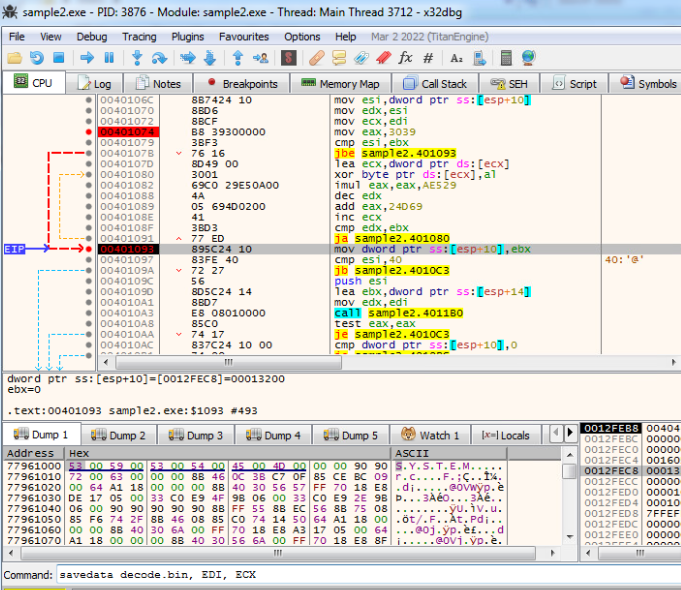
\includegraphics[width=\textwidth]{decode.png}
        \caption{Saving the decoded resource data from x32dbg with the "savedata" command}
    \end{figure}
    
    This new executable does not set or create any registry keys, but it does write to the same places as sample2.exe. Except it does not write to the "systemprofile" directory. However, this program has more networking traffic and contains different imports.
    \pagebreak
    \section{Indicators of Compromise}
    \subsection{Host Indicators}
    sample2.exe is running, and the following files are present:
    \begin{itemize}
        \item \path{C:\Users\System32\config\systemprofile\AppData\Roaming\client_id}
        \item MD5: FD6B35B511CBC03CBCCD989173A34CCC
        \item \path{C:\Users\System32\config\systemprofile\AppData\Roaming\group_tag}
        \item MD5: 84EC10941396194167183E29FFD32D41
        \item \path{C:\Users\System32\config\systemprofile\AppData\Roaming\sample2.exe}
        \item MD5: E05D85ACC62B2795BFB94A681E64E20F
    \end{itemize}
    \subsection{Network Indicators}
    The connections to the following:
    \begin{itemize}
        \item HTTP GET \url{http://myexternalip.com/raw}
        \item TCP and DNS request \url{in-addr.arpa}
    \end{itemize}
    \subsection{Yara Rule}
    \begin{verbatim}
import "pe"

rule sample2 {
    meta:
        author = "Michael Ivanov"
    strings:
        $s1 = "Wow64DisableWow64FsRedirection" fullword ascii
        $s2 = "NtQueryInformationProcess" fullword ascii
        $s3 = "GetProcAddress" fullword ascii
        $s4 = "IDR_X86BOT" fullword ascii
    condition:
        uint16(0) == 0x5A4D
        and $s1 and $s2 and $s3 and $s4
}
    \end{verbatim}
    \pagebreak
    \printbibliography

\end{document}